\section{Methods}
\label{sec:method}

\subsection{Problem Setup}
\label{subsec:problem_setup}

Given a degraded old-film clip $X=\{x_t\}_{t=1}^{T}$, we aim to recover a clean clip $Y=\{y_t\}_{t=1}^{T}$ with restored image content and reduced structured film defects and photometric degradation. Synthetic SRWOV clips provide paired clean frames for direct supervision. Real-world archival clips have no ground truth, so we evaluate them with no-reference quality metrics and qualitative inspection. Old-film degradations vary over both spatial scale and time, and a restoration model must remove them without breaking temporal consistency.

\subsection{Input Representation}
\label{subsec:input_representation}

Each input frame is an RGB image, and the baseline propagation module converts the clip into backward and forward feature streams. At each time step $t$, motion-aware propagation yields aligned feature maps $f_t^{b}, f_t^{f} \in \mathbb{R}^{C_f \times H \times W}$. MgfrOFR operates entirely on these propagated maps: MGFE takes each map, returns a recalibrated map with the same spatial size and channel count, and produces the branch descriptors used by RATR during training.

MgfrOFR retains the bidirectional propagation framework of MambaOFR~\cite{mao2025mambaofr} but replaces its single-granularity restoration view with an explicit coarse-to-fine pipeline. Given the degraded clip $X=\{x_t\}_{t=1}^{T}$, the baseline first propagates content backward and forward so that neighboring frames are motion-aligned before restoration, and MgfrOFR builds on these aligned features. Old-film damage is spatially and temporally asymmetric: a scratch may cover one region in one frame and vanish in the next, yet restoration should still balance coarse, medium, and fine evidence. This cross-granularity balance is the feature-space symmetry targeted by our design.

MGFE turns each propagated feature map into a token sequence, inserts learnable restoration tokens, and reads branch descriptors from progressively fused token groups; their summaries flow back to the propagated feature through channel-wise recalibration. RATR acts only during training, where it discourages branches from inducing the same temporal rankings, and is disabled at inference. The reconstruction head is inherited unchanged from MambaOFR and outputs the restored frame. Figure~\ref{fig:architecture} shows how these components fit together.

\begin{figure}[!htbp]
\centering
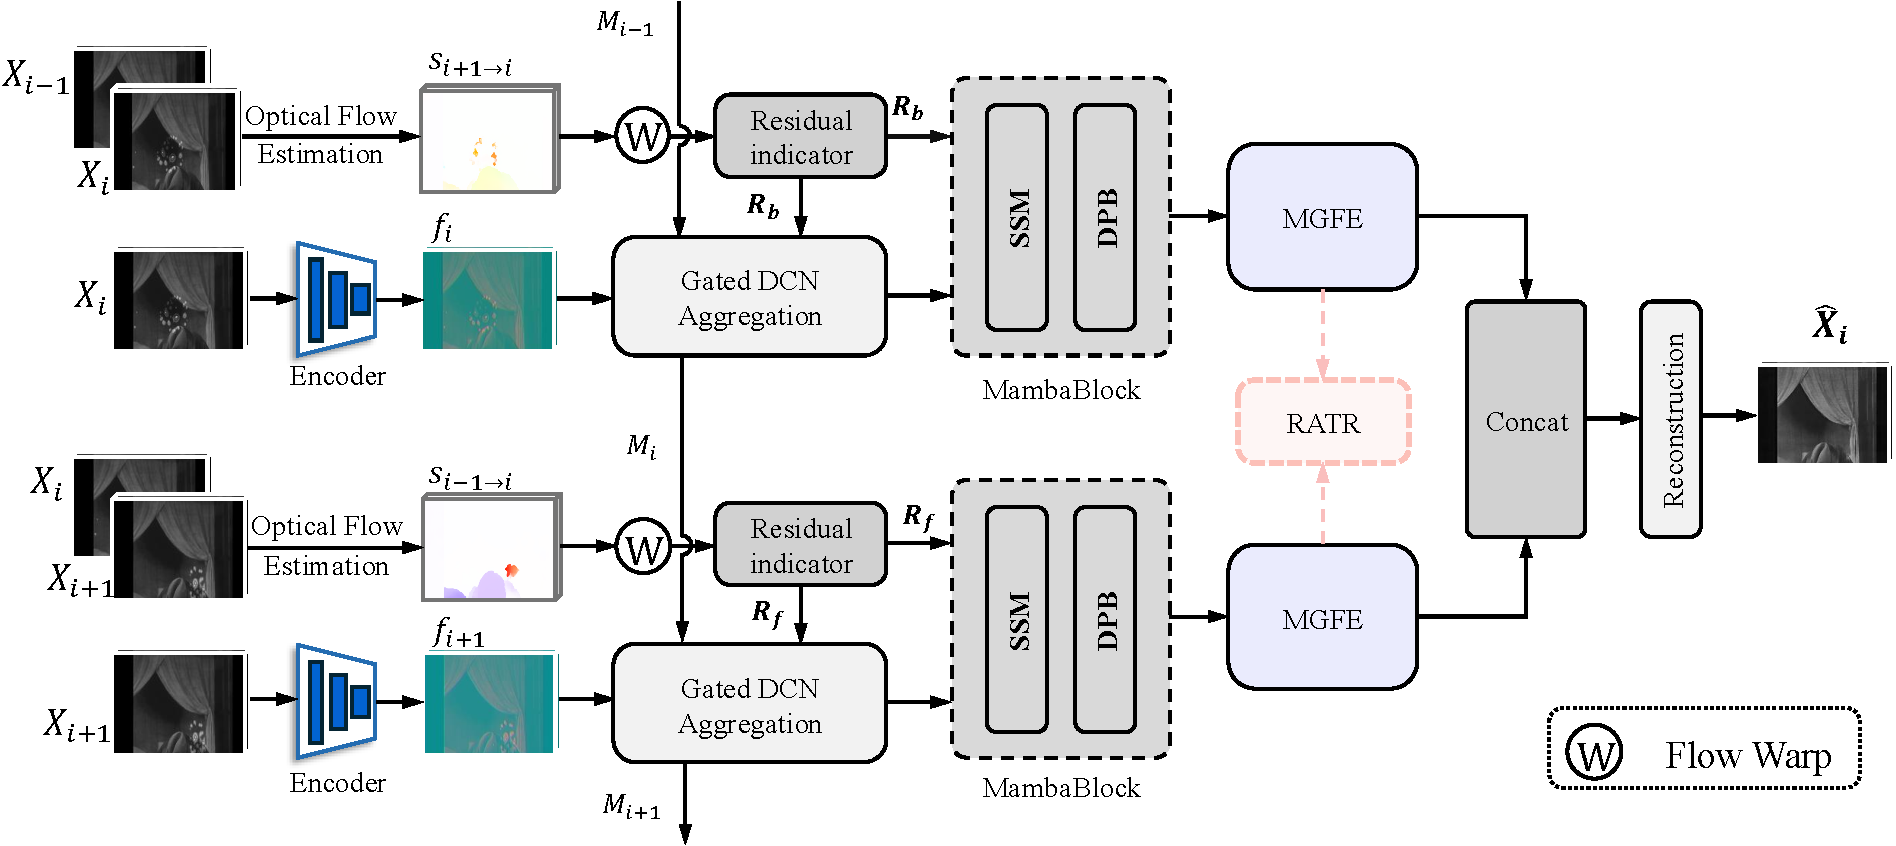
\includegraphics[width=\textwidth]{figures/Fig1_mgfrofr_architecture.pdf}
\caption{Overview of the MgfrOFR framework. MGFE decomposes propagated features into $G{=}3$ multi-granularity restoration-token branches for channel-wise recalibration. RATR is used only during training (dashed red path) to penalize redundant temporal-ranking correlations and produce $\mathcal{L}_{\text{intra}}$ and $\mathcal{L}_{\text{inter}}$.\label{fig:architecture}}
\end{figure}

\subsection{Pipeline Overview}
\label{subsec:overview}

At time step $t$, the baseline provides propagated maps $f_t^{b}, f_t^{f} \in \mathbb{R}^{C_f \times H \times W}$, and MGFE maps each one to a recalibrated feature map together with a set of branch descriptors:

\begin{equation}
\left(\widetilde{f}_t^{d}, B_t^{d}\right)=\operatorname{MGFE}\!\left(f_t^{d}\right), \quad d \in \{b,f\},
\end{equation}

where $d$ indexes the propagation direction, $B_t^{d} \in \mathbb{R}^{G \times D}$ is the branch-descriptor tensor, and $D=C_f$ in this work. The reconstruction head keeps the original MambaOFR interface and combines the two recalibrated directional features:

\begin{equation}
y_t = \mathcal{R}\!\left([\widetilde{f}_t^{b};\widetilde{f}_t^{f}], x_t\right),
\qquad
B_t = \frac{1}{2}\left(B_t^{b}+B_t^{f}\right),
\label{eq:mgfrofr_overview_2}
\end{equation}

where $\mathcal{R}(\cdot)$ is the unchanged reconstruction head of MambaOFR and $[\cdot;\cdot]$ denotes channel concatenation. Averaging the two directional descriptors before RATR, as in Equation~\eqref{eq:mgfrofr_overview_2}, lets the diversity regularizer operate on a single descriptor tensor per frame instead of two nearly identical streams. Figure~\ref{fig:architecture} traces this data flow, and Algorithm~\ref{alg:mgfrofr} summarizes the forward pass.

\begin{algorithm}[H]
\caption{MgfrOFR forward pass for a clip of length $T$.\label{alg:mgfrofr}}
\begin{algorithmic}[1]
\Require Degraded clip $X=\{x_t\}_{t=1}^{T}$
\Ensure Restored frames $\{y_t\}_{t=1}^{T}$
\State Initialize descriptor buffer $\mathcal{B} \leftarrow \emptyset$
\For{$t = 1$ to $T$}
    \State $f_t^{b}, f_t^{f} \leftarrow \text{Backbone}(X, t)$ \Comment{Bidirectional propagation}
    \For{$d \in \{b, f\}$}
        \State $\widetilde{f}_t^{d}, B_t^{d} \leftarrow \text{MGFE}(f_t^{d})$ \Comment{Multi-granularity decomposition}
    \EndFor
    \State $B_t \leftarrow \frac{1}{2}(B_t^{b} + B_t^{f})$ \Comment{Average branch descriptors}
    \State $\mathcal{B} \leftarrow \mathcal{B} \cup \{B_t\}$ \Comment{Accumulate into batch buffer}
    \State $y_t \leftarrow \mathcal{R}([\widetilde{f}_t^{b}; \widetilde{f}_t^{f}], x_t)$ \Comment{Reconstruction}
\EndFor
\If{training}
    \State $\mathcal{L}_{\text{ratr}} \leftarrow \text{RATR}(\{B_t\}_{t=1}^{T})$ \Comment{Applied on full batch after accumulation}
    \State $\mathcal{L}_{\text{total}} \leftarrow \mathcal{L}_{\text{pix}} + \lambda_{\text{perc}}\mathcal{L}_{\text{perc}} + \lambda_{\text{gan}}\mathcal{L}_{\text{gan}} + \lambda_{\text{ratr}}\mathcal{L}_{\text{ratr}}$
\EndIf
\end{algorithmic}
\end{algorithm}

\subsection{Baseline Interface and Preserved Components}
\label{subsec:baseline_interface}

MgfrOFR leaves the MambaOFR backbone, propagation order, reconstruction head, and training loop unchanged. At inference, the only addition is MGFE, which maps $f_t^{d}$ to $\widetilde{f}_t^{d}$ without changing the tensor shape; RATR is an auxiliary loss on the branch descriptors and plays no role once training ends. The reconstruction head therefore behaves as in the baseline, still taking the concatenated backward and forward features together with the current degraded frame.

\subsection{Multi-Granularity Feature Extractor (MGFE)}
\label{subsec:mgfe}

Old films are damaged at very different scales: large missing regions, mid-scale blotches, and thin scratches each require a different aggregation range. A single restoration feature must serve all of them at once, so fine detail and coarse structure compete inside the same channels. MGFE addresses this conflict by keeping the propagated feature as a shared spatial carrier while exposing several restoration-token branches that aggregate at different rates; the branch summaries are fed back to the carrier as a recalibration signal. Each damage scale therefore receives a dedicated branch, while reconstruction still reads from one common feature. Figure~\ref{fig:mgfe_detail} details the design.

\begin{figure}[!htbp]
\centering
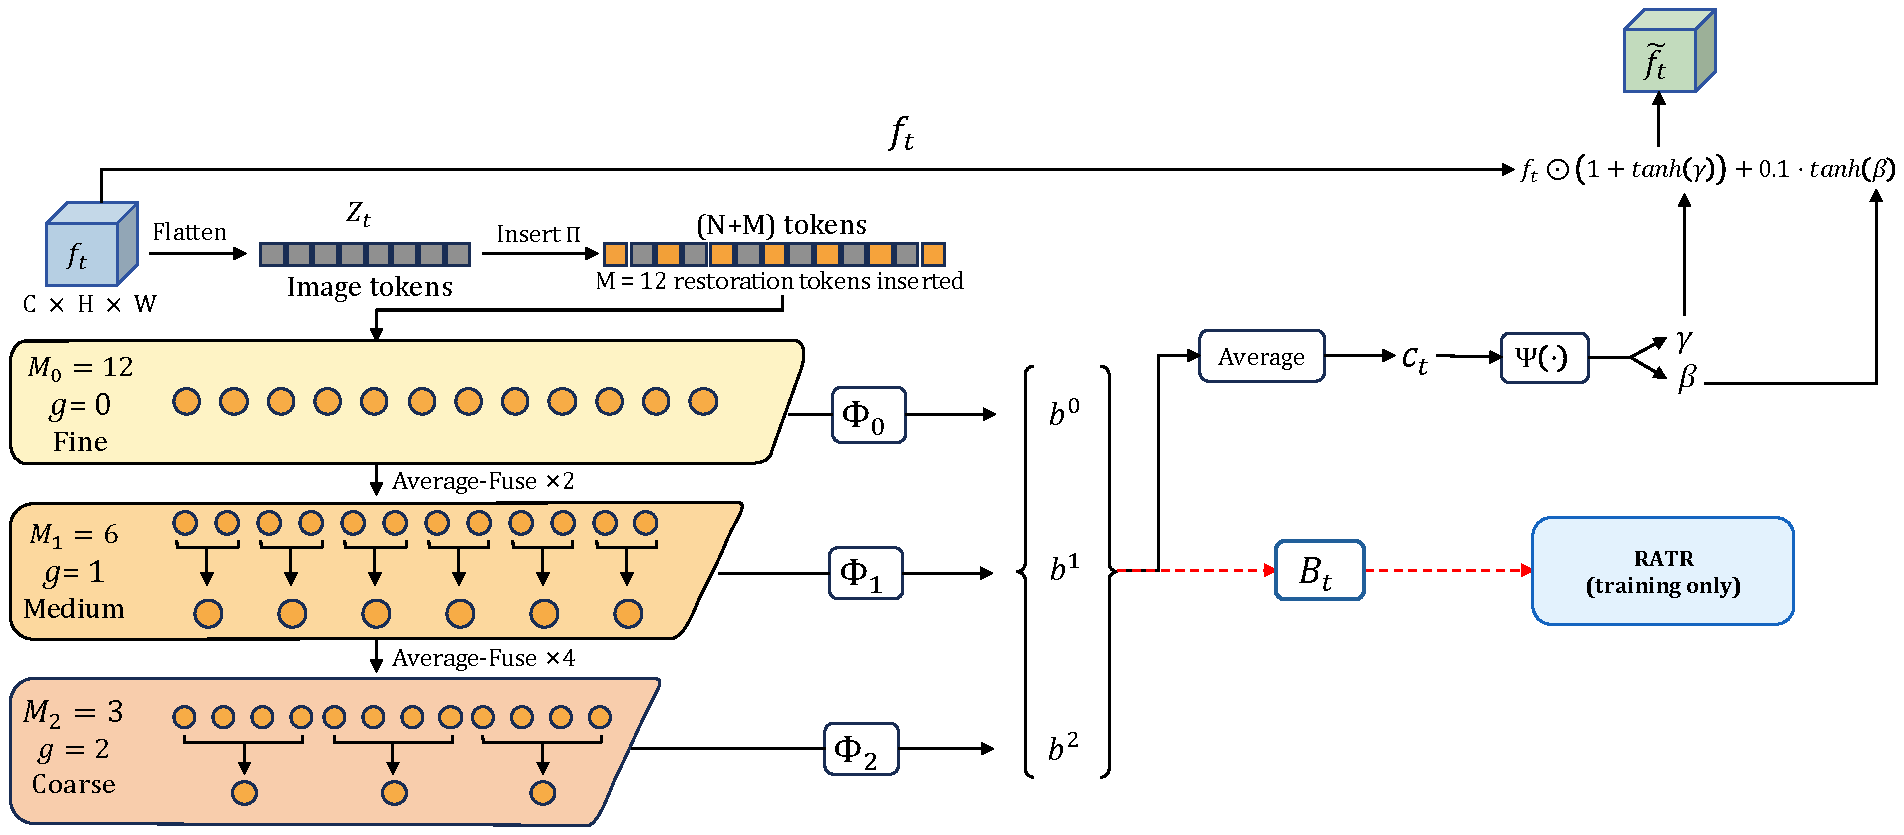
\includegraphics[width=\textwidth]{figures/Fig2_mgfe_module_detail.pdf}
\caption{Detailed MGFE module. Propagated features are decomposed into $G{=}3$ restoration-token branches. $M{=}12$ learnable restoration tokens are inserted into image tokens, fused by progressive average fusion, and summarized into descriptors that generate scale/shift parameters for channel-wise recalibration.\label{fig:mgfe_detail}}
\end{figure}

Since MGFE processes each propagation direction identically, we drop the direction superscript $d$ and write $f_t \in \mathbb{R}^{C_f \times H \times W}$ for brevity. We first flatten it into an image-token sequence

\begin{equation}
Z_t = \operatorname{Flat}(f_t) \in \mathbb{R}^{N \times C_f},
\qquad
N = H W,
\end{equation}

where $\operatorname{Flat}(\cdot)$ preserves raster order and stacks spatial positions as tokens. We append $M$ learnable restoration tokens $R \in \mathbb{R}^{M \times C_f}$ and insert them into the image-token stream through an operator $\Pi(\cdot,\cdot)$. The restoration-token matrix is initialized from a truncated normal distribution with standard deviation 0.02 and optimized jointly with the restoration network:

\begin{equation}
\widehat{Z}_t = \Pi(Z_t, R) \in \mathbb{R}^{(N+M)\times C_f}.
\end{equation}

The insertion $\Pi$ partitions the $N$ image tokens into $M{+}1$ approximately equal chunks and places one restoration token after each of the first $M$ chunks, keeping the original image-token order. Each chunk receives $\lfloor N/(M{+}1)\rfloor$ or $\lceil N/(M{+}1)\rceil$ image tokens, so the total remains exactly $N$. For example, with $M=3$ and $N=9$ the four chunks hold $\{3,2,2,2\}$ image tokens and the three restoration tokens land at cumulative positions $\{3,6,9\}$ in the 12-token interleaved sequence. Spacing the tokens uniformly in this way gives them balanced receptive ranges over the full spatial support.

MGFE then builds $G$ granularity branches by progressively fusing restoration tokens, following the progressive fusion scheme introduced in ReIDMamba~\cite{gu2025reidmamba} and adapting it to spatial restoration features. To make every branch well defined, the number of restoration tokens must satisfy the divisibility constraint
\begin{equation}
M = k \cdot 2^{G-1},\quad k \in \mathbb{N}^{+},
\end{equation}
so that every branch size $M_g = M/2^g$ is an integer for $g\in\{0,\ldots,G-1\}$. We use $G=3$ and $M=12$ ($k=3$) throughout; see Section~\ref{subsec:sensitivity} for alternative configurations.

For branch $g \in \{0,\ldots,G-1\}$, MGFE fuses restoration tokens with a sampling rate of $2^g$. The fused restoration tokens are defined as

\begin{equation}
R^{(g)}[j] =
\mathcal{F}\!\left(
\left\{R[j{\cdot}2^g+k]\right\}_{k=0}^{2^g-1}
\right),\quad
j = 0,\ldots,M_g-1,
\end{equation}

where $\mathcal{F}(\cdot)$ denotes an element-wise average over all tokens in the fusion group:

\begin{equation}
\mathcal{F}\!\left(
\left\{R[j\cdot2^g+k]\right\}_{k=0}^{2^g-1}
\right)
= \frac{1}{2^g}\sum_{k=0}^{2^g-1} R[j\cdot2^g+k]\;\in\mathbb{R}^{C_f}.
\label{eq:avg_fusion}
\end{equation}

The average is taken channel-wise. We use average fusion in the main MgfrOFR configuration because it keeps all restoration tokens contributing to the branch descriptor and prevents a single high-response token from dominating the recalibration signal. The max-fusion variant is retained as a control in Section~\ref{subsec:ablation}; its lower full-reference scores motivate average fusion as the default. A smaller $g$ keeps more tokens and preserves fine local detail; a larger $g$ pools a wider support and emphasizes coarse context.

The fused tokens are re-inserted into the same image-token sequence using the same uniform-spacing insertion rule:

\begin{equation}
\widehat{Z}_t^{(g)} = \Pi\!\left(Z_t,R^{(g)}\right),
\end{equation}

and the resulting sequence is processed by a lightweight branch-specific token mixer $\Phi_g(\cdot)$:

\begin{equation}
U_t^{(g)} = \Phi_g\!\left(\widehat{Z}_t^{(g)}\right)
\in \mathbb{R}^{(N+M_g)\times C_f},
\end{equation}

where $M_g = M/2^g$. Each $\Phi_g$ consists of two sequential linear-complexity token blocks, and each block contains a context-augmented projection sublayer and a feed-forward sublayer. The projection sublayer first applies LayerNorm, computes a global context vector by mean pooling over the token dimension, and adds it (through a learned linear projection) to the per-token linear projection, followed by a residual connection. The feed-forward sublayer applies LayerNorm followed by a two-layer MLP with GELU activation and hidden dimension $2C_f$, again with a residual connection. Formally, for input tokens $\mathbf{h}$, each block computes
\begin{equation}
\mathbf{h}' = \mathbf{h} + W_t\,\mathrm{LN}(\mathbf{h}) + W_c\,\overline{\mathrm{LN}(\mathbf{h})},\qquad
\mathbf{h}'' = \mathbf{h}' + \mathrm{MLP}(\mathrm{LN}(\mathbf{h}')),
\end{equation}
where $\overline{(\cdot)}$ denotes mean pooling over the token dimension, $W_t,W_c\in\mathbb{R}^{C_f\times C_f}$ are learned projections, and MLP consists of $\mathrm{Linear}(C_f\!\rightarrow\!2C_f)\!\rightarrow\!\mathrm{GELU}\!\rightarrow\!\mathrm{Linear}(2C_f\!\rightarrow\!C_f)$. The global context term $W_c\,\overline{\mathrm{LN}(\mathbf{h})}$ gives every token an inexpensive summary of the whole sequence, so tokens exchange information at linear cost. Each branch owns its pair of token blocks and can specialize to its granularity; because the blocks are small, the extra parameter count remains modest.

After branch processing, we summarize each branch by averaging the updated restoration-token positions:

\begin{equation}
b_t^{(g)} =
\frac{1}{M_g}
\sum_{m=1}^{M_g}
U_t^{(g)}[\pi_m^{(M_g)}]
\in \mathbb{R}^{D},
\end{equation}

where $\{\pi_m^{(M_g)}\}_{m=1}^{M_g}$ denote the uniformly spaced insertion positions for $M_g$ tokens, and $D=C_f$. Stacking all branch descriptors gives

\begin{equation}
B_t =
\left[
b_t^{(0)}, b_t^{(1)}, \ldots, b_t^{(G-1)}
\right]^\top
\in \mathbb{R}^{G \times D}.
\end{equation}

Because all descriptors come from the same propagated feature but at different fusion rates, they remain semantically aligned while differing in granularity. RATR later operates on this descriptor tensor $B_t$.

MGFE further converts the branch descriptors into a channel-wise recalibration signal. We first average the branch context,

\begin{equation}
c_t = \frac{1}{G}\sum_{g=0}^{G-1}b_t^{(g)},
\qquad
[\boldsymbol{\gamma}_t,\boldsymbol{\beta}_t] = \Psi(c_t),
\label{eq:recalibration_context}
\end{equation}

where $\Psi(\cdot)$ is a projection head consisting of $\mathrm{LayerNorm}\!\rightarrow\!\mathrm{Linear}(C_f\!\rightarrow\!2C_f)\!\rightarrow\!\mathrm{GELU}\!\rightarrow\!\mathrm{Linear}(2C_f\!\rightarrow\!2C_f)$ that outputs concatenated scale and shift vectors. The recalibrated propagated feature is then

\begin{equation}
\widetilde{f}_t =
f_t \odot
\left(1+\tanh(\boldsymbol{\gamma}_t)\right)
+ 0.1\,\tanh(\boldsymbol{\beta}_t),
\label{eq:recalibration}
\end{equation}

where the vectors from Equation~\eqref{eq:recalibration_context} are broadcast over the spatial dimensions. The multiplicative term $(1+\tanh(\boldsymbol{\gamma}_t))$ starts near unity, and the small additive coefficient $0.1$ caps the shift at about $10\%$ of the $\tanh$ range, following the conservative residual scaling of FiLM-style modulation~\cite{perez2018film}. The recalibrated feature therefore stays close to the propagated feature while the branch context remains uninformative, allowing the model to reproduce baseline behavior early in training. As the descriptors sharpen, the coarse branches emphasize global structure and the fine branches highlight local damage.

MGFE produces two outputs from the same propagated feature: the branch descriptors $B_t$ and the recalibration signal $(\boldsymbol{\gamma}_t, \boldsymbol{\beta}_t)$. The descriptors feed the ranking regularizer of Section~\ref{subsec:ratr}, while the recalibration modulates the propagated feature by granularity. Keeping them separate lets us switch off recalibration without changing the descriptors, as in the RATR-only configuration of Section~\ref{subsec:ablation}. Explicit branches, however, do not guarantee complementary features. If every branch ranks samples in the same order, the branches collapse into redundant descriptors, which motivates the regularizer below.

\subsection{Ranking-Aware Triplet Regularization (RATR)}
\label{subsec:ratr}

RATR keeps the branches from collapsing by penalizing how strongly their rankings agree. Descriptor orthogonality alone is insufficient: two branches can be orthogonal yet still order the same samples identically, leaving them redundant and undermining the balance created by MGFE. The ordering is therefore the target. For an anchor frame compared with nearby positives and harder negatives, RATR measures whether two branches rank that candidate set alike, using Kendall's~\cite{kendall1938measure} rank correlation coefficient made differentiable by DiffKendall~\cite{zheng2023diffkendall}. Figure~\ref{fig:ratr_detail} shows the workflow.

\begin{figure}[!htbp]
\centering
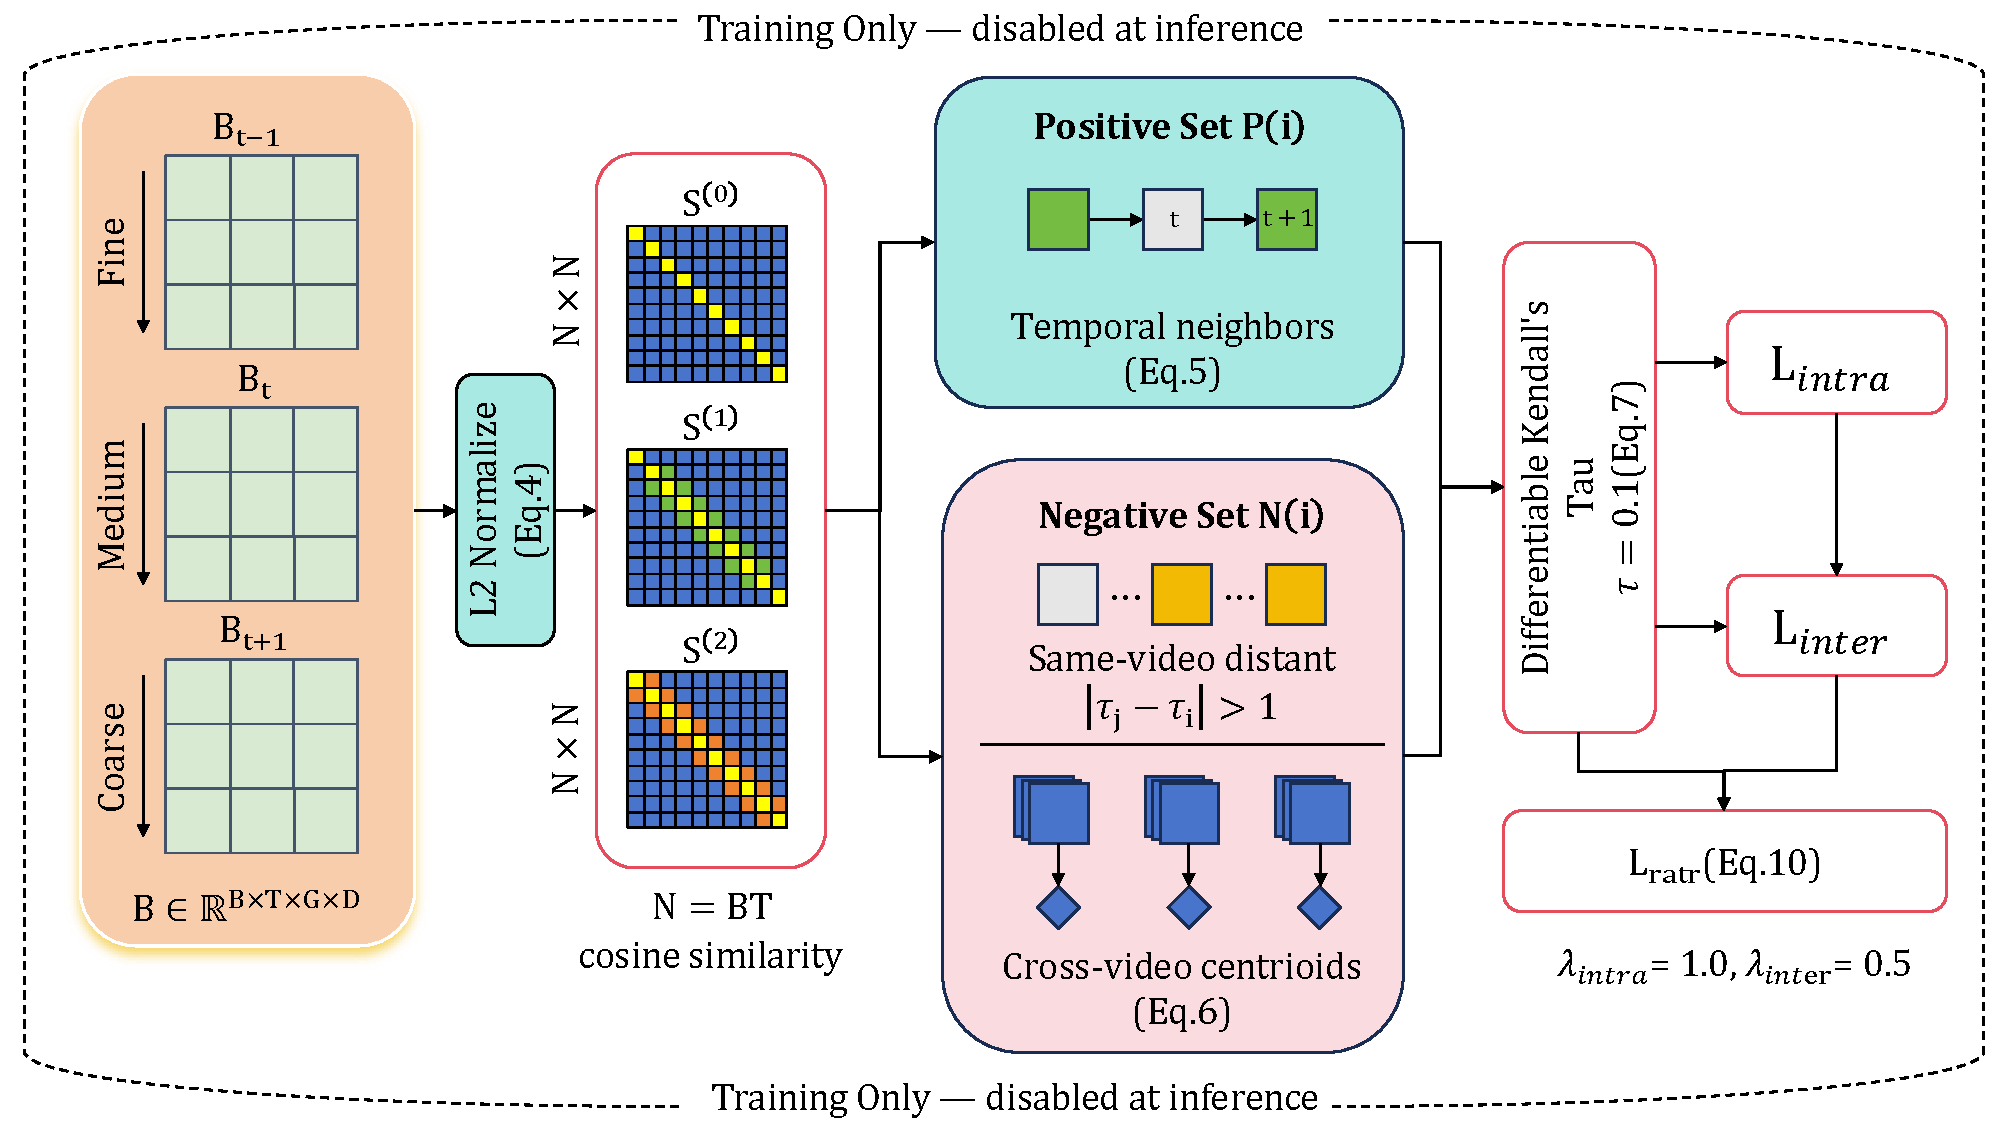
\includegraphics[width=\textwidth]{figures/Fig3_ratr_module_detail.pdf}
\caption{RATR compares branch-specific ranking sequences from temporal correspondences using differentiable Kendall's Tau. Neighboring frames define positives, while distant same-video frames and cross-video centroids define negatives, producing $\mathcal{L}_{\text{intra}}$ and $\mathcal{L}_{\text{inter}}$ during training only.\label{fig:ratr_detail}}
\end{figure}

Let the averaged branch descriptors from Equation~\eqref{eq:mgfrofr_overview_2} be organized as a 4D tensor of shape $N_b\times T\times G\times D$, where $N_b$ is the batch size. We flatten batch and time into $\bar{N}=N_b T$ samples and normalize the descriptors branch-wise:

\begin{equation}
\widehat{b}_i^{(g)} =
\frac{b_i^{(g)}}{\|b_i^{(g)}\|_2},
\qquad
i=1,\ldots,\bar{N}.
\end{equation}

For each branch $g$, we compute a cosine-similarity matrix

\begin{equation}
\mathcal{S}^{(g)}[i,j] =
\left\langle
\widehat{b}_i^{(g)},
\widehat{b}_j^{(g)}
\right\rangle.
\end{equation}

This matrix supplies the rankings rather than serving as a supervision target itself: each anchor draws one positive ranking sequence and one negative ranking sequence from it, forming the anchor-positive-negative triplet that RATR regularizes.

For anchor $i$, the positive set is defined from temporal correspondences within the same clip:

\begin{equation}
\mathcal{P}(i)=
\bigl\{
j \mid v_j=v_i,\;
|t_j-t_i|=1
\bigr\},
\end{equation}

where $v_i$ and $t_i$ are the clip and frame indices of sample $i$. Adjacent frames are natural positives because the flow-guided deformable alignment in MambaOFR has already warped neighboring frames onto the anchor before MGFE runs; after alignment, they are the most reliable feature-domain proxy for true correspondences. Because $|\mathcal{P}(i)| \le 2$ (at most one predecessor and one successor), boundary frames have only a single positive neighbor, and we compute the intra-ranking term only on anchors that have at least two positives:
\begin{equation}
\mathcal{I}_{\text{intra}}=
\bigl\{
i \mid |\mathcal{P}(i)| \ge 2
\bigr\}.
\end{equation}
For the seven-frame clips used in training, this excludes only the first and last frame of each clip, and every interior anchor contributes one pairwise ordering comparison to $\mathcal{L}_{\text{intra}}$. In practice, $\mathcal{L}_{\text{intra}}$ is averaged over many valid anchors per batch, while $\mathcal{L}_{\text{inter}}$ adds a complementary signal from the richer negative set.

Negative evidence is drawn from two harder sources: temporally distant frames inside the same clip and clip-level representatives from other clips. The same-video negatives are

\begin{equation}
\mathcal{N}_{sv}(i)=
\bigl\{
j \mid v_j=v_i,\;
|t_j-t_i|>1
\bigr\},
\end{equation}

and the clip-level centroid for another video $v\neq v_i$ is

\begin{equation}
\bar{b}_{v}^{(g)} =
\frac{1}{|\mathcal{T}_v|}
\sum_{t\in\mathcal{T}_v}
\widehat{b}_{(v,t)}^{(g)},
\end{equation}

where $\mathcal{T}_v$ denotes the set of frame indices in clip $v$. We then construct the negative ranking sequence as

\begin{equation}
\bar{\mathcal{S}}_i^{(g)} =
\Bigl[\mathcal{S}^{(g)}[i,j]\Bigr]_{j\in\mathcal{N}_{sv}(i)}
\oplus
\Bigl[\bigl\langle \widehat{b}_i^{(g)},\,\bar{b}_v^{(g)} \bigr\rangle\Bigr]_{v\neq v_i},
\end{equation}

where $\oplus$ denotes sequence concatenation. Distant frames from the same clip are hard negatives: they share content and degradation with the anchor but are no longer immediate neighbors. Using one centroid per other clip gives a stable clip-level negative and keeps the cost linear instead of incurring the $O(\bar{N}^2)$ cost of comparing every cross-clip frame pair.

To compare how two branches rank the same candidate set, we adopt a differentiable version of Kendall's Tau. For sequences $p,q\in\mathbb{R}^{L}$, the differentiable statistic is

\begin{equation}
\mathrm{DKTau}(p,q;\tau)
= \frac{1}{\binom{L}{2}}
\sum_{1\le u < v \le L}
\tanh\!\!\left(\frac{p_u-p_v}{\tau}\right)
\cdot
\tanh\!\!\left(\frac{q_u-q_v}{\tau}\right),
\label{eq:dktau}
\end{equation}

where $\tau>0$ is a temperature parameter. As $\tau\rightarrow 0$, Equation~\eqref{eq:dktau} approaches the hard sign comparison used in the exact Kendall coefficient; as $\tau$ becomes too large, pairwise order differences are oversmoothed and gradients vanish. We set $\tau=0.1$ (see Section~\ref{subsec:sensitivity} for the sensitivity to this choice). A lower value of $\mathrm{DKTau}(p,q;\tau)$ indicates weaker ranking correlation between branches and therefore stronger branch complementarity.

Using Equation~\eqref{eq:dktau}, we compute the positive-ranking correlation loss as

\begin{equation}
\mathcal{L}_{\text{intra}} =
\frac{1}{|\mathcal{I}_{\text{intra}}| \binom{G}{2}}
\sum_{i\in\mathcal{I}_{\text{intra}}}
\sum_{g < g'}
\mathrm{DKTau}\!\Bigl(
\mathcal{S}^{(g)}[i,\mathcal{P}(i)],\,
\mathcal{S}^{(g')}[i,\mathcal{P}(i)];\,\tau
\Bigr),
\label{eq:loss_intra}
\end{equation}

and the negative-ranking correlation loss as

\begin{equation}
\mathcal{L}_{\text{inter}} =
\frac{1}{\bar{N} \binom{G}{2}}
\sum_{i=1}^{\bar{N}}
\sum_{g < g'}
\mathrm{DKTau}\!\Bigl(
\bar{\mathcal{S}}_i^{(g)},\,
\bar{\mathcal{S}}_i^{(g')};\,
\tau
\Bigr).
\end{equation}

The final ranking-aware regularizer is

\begin{equation}
\mathcal{L}_{\text{ratr}} =
\lambda_{\text{intra}}\,\mathcal{L}_{\text{intra}}
+ \lambda_{\text{inter}}\,\mathcal{L}_{\text{inter}}.
\label{eq:loss_ratr}
\end{equation}

Equations~\eqref{eq:loss_intra}--\eqref{eq:loss_ratr} are complementary: the intra term prevents two branches from ordering the most reliable temporal correspondences the same way, and the inter term prevents the same collapse on harder negatives. Neither term drives the branches toward meaningless disagreement, because the reconstruction losses still tie every branch to the same target through MGFE.

\subsection{Symmetry Property of the Regularizer}
\label{subsec:symmetry_property}

The representation symmetry introduced in Section~\ref{sec:introduction} has a concrete meaning in MgfrOFR. It is not a geometric symmetry of the image content but an invariance of the diversity objective under group actions that relabel branches or exchange propagation directions. Two such invariances hold, and together they explain why the constraint is a symmetry principle rather than a balancing heuristic, as discussed in Section~\ref{subsec:symmetry_ai}.

\textbf{Property 1 (Branch-permutation invariance).} Both the intra term in Equation~\eqref{eq:loss_intra} and the inter term $\mathcal{L}_{\text{inter}}$ sum the differentiable Kendall statistic over unordered branch pairs $g<g'$, and Equation~\eqref{eq:dktau} is symmetric in its arguments, $\mathrm{DKTau}(p,q;\tau)=\mathrm{DKTau}(q,p;\tau)$. Permuting the branch index of every descriptor by the same $\pi$ therefore leaves the regularizer unchanged:
\begin{equation}
\mathcal{L}_{\text{ratr}}\!\left(\{b^{(g)}\}_{g=0}^{G-1}\right)
=
\mathcal{L}_{\text{ratr}}\!\left(\{b^{(\pi(g))}\}_{g=0}^{G-1}\right),
\qquad
\forall\,\pi\in\mathcal{S}_G,
\label{eq:branch_permutation}
\end{equation}
where $\mathcal{S}_G$ is the symmetric group on the $G$ branches. In other words, $\mathcal{L}_{\text{ratr}}$ depends only on the unordered set of pairwise branch relations, not on any branch ordering or index. Because $\mathcal{S}_G$ has no privileged element, the objective does not assign a preferred role to any branch.

\textbf{Property 2 (Direction-exchange invariance).} The two propagation streams enter the regularizer only through the average $B_t=\tfrac{1}{2}(B_t^{b}+B_t^{f})$ in Equation~\eqref{eq:mgfrofr_overview_2}, which is invariant under the $\mathbb{Z}_2$ action that swaps the backward and forward descriptors, $B_t^{b}\!\leftrightarrow\!B_t^{f}$. The objective thus treats the two temporal directions symmetrically and inherits the bidirectional symmetry of the backbone.

\textbf{Symmetry versus balancing.} These two invariances separate our constraint from a tuned balancing term. Balancing targets an \emph{outcome} (branches that end up contributing comparably) and is usually enforced by an asymmetric, hand-weighted penalty on individual branch magnitudes. RATR instead is built from group-invariant quantities ($\mathcal{S}_G$ on branches, $\mathbb{Z}_2$ on directions) and applies the identical constraint to every branch by construction. Balanced, complementary branches follow as a \emph{consequence} of optimizing this symmetric objective, not as a separately weighted goal.

\textbf{Scope of the claim.} The symmetry here is functional and representation-level: an invariance of the learning objective under permutation and exchange group actions, both standard symmetry principles in machine learning, rather than a visible geometric symmetry of the restored frames. We keep this reading deliberately narrow, and Section~\ref{subsec:symmetry_ai} relates it to the broader use of symmetry in representation learning.

\subsection{Training Objective}
\label{subsec:training_objective}

The generator objective combines the standard old film restoration losses used by the MambaOFR baseline with our ranking-aware regularizer. We use an $L_1$ pixel reconstruction loss $\mathcal{L}_{\mathrm{pix}}$, whose robustness for image restoration is analyzed in~\cite{zhao2017loss_restoration}, a VGG-based perceptual loss $\mathcal{L}_{\mathrm{perc}}$~\cite{johnson2016perceptual}, an adversarial loss $\mathcal{L}_{\mathrm{gan}}$~\cite{goodfellow2014gan}, and the ranking regularizer $\mathcal{L}_{\mathrm{ratr}}$:

\begin{equation}
\mathcal{L}_{\mathrm{total}} =
\mathcal{L}_{\mathrm{pix}}
+ \lambda_{\mathrm{perc}}\mathcal{L}_{\mathrm{perc}}
+ \lambda_{\mathrm{gan}}\mathcal{L}_{\mathrm{gan}}
+ \lambda_{\mathrm{ratr}}\mathcal{L}_{\mathrm{ratr}}.
\label{eq:loss_total}
\end{equation}

Because MGFE only augments the propagated feature stream and RATR is a pure auxiliary term, Equation~\eqref{eq:loss_total} fits into the baseline training loop without any other change. We set $\lambda_{\mathrm{perc}}=1.0$ and $\lambda_{\mathrm{gan}}=0.01$, following RTN~\cite{wan2022rtn} and MambaOFR~\cite{mao2025mambaofr}, and use $\lambda_{\mathrm{ratr}}=0.1$, $\lambda_{\mathrm{intra}}=1.0$, and $\lambda_{\mathrm{inter}}=0.5$ for the ranking term (see Section~\ref{subsec:sensitivity}). The smaller weight on $\mathcal{L}_{\text{inter}}$ reflects the coarser ordering signal from clip-centroid negatives. Unless stated otherwise, the full model uses feature dimension $C_f=16$, $G=3$ branches, $M=12$ restoration tokens, channel-wise average fusion in Equation~\eqref{eq:avg_fusion}, and differentiable Kendall temperature $\tau=0.1$.
